\subsection{Closed Loop}
\label{sec:closed_loop}
\begin{figure*}
\centering
%\vspace*{-0.3cm}  
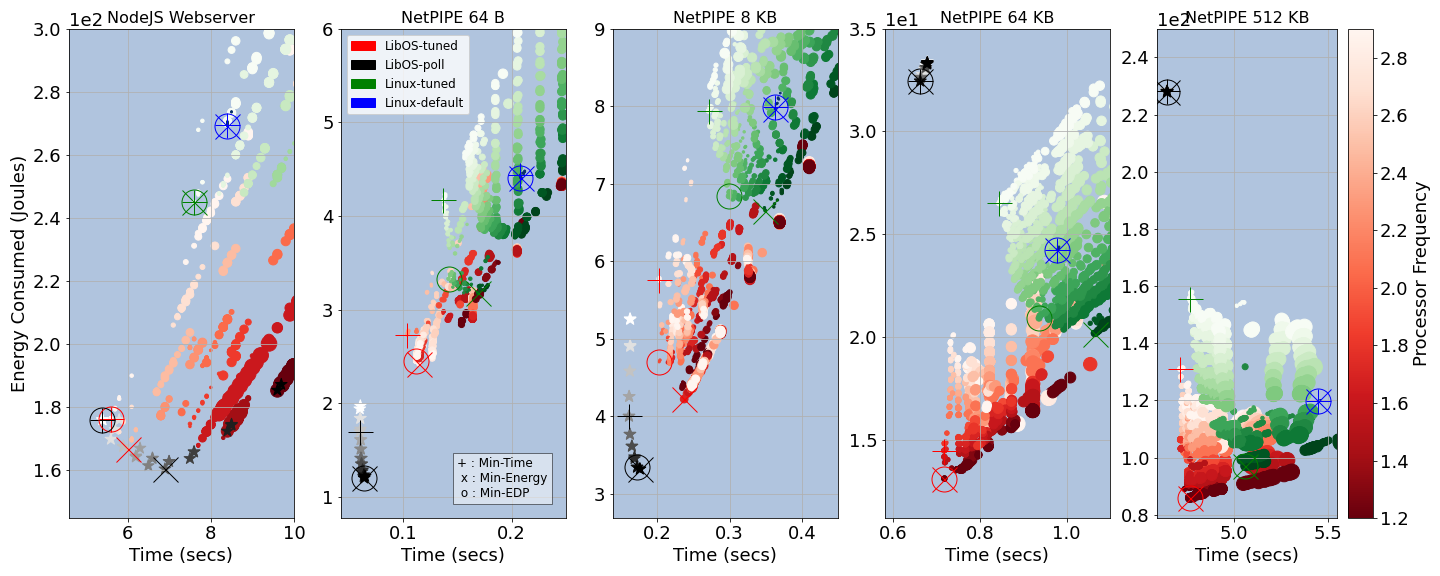
\includegraphics[width=1\textwidth]{figures/closed_loop_overview.png}
\caption[]
%{\small 
{Closed loops.}
\label{fig:closed_loop_overview}
\end{figure*}
\begin{figure*}
\centering
%\vspace*{-0.3cm}  
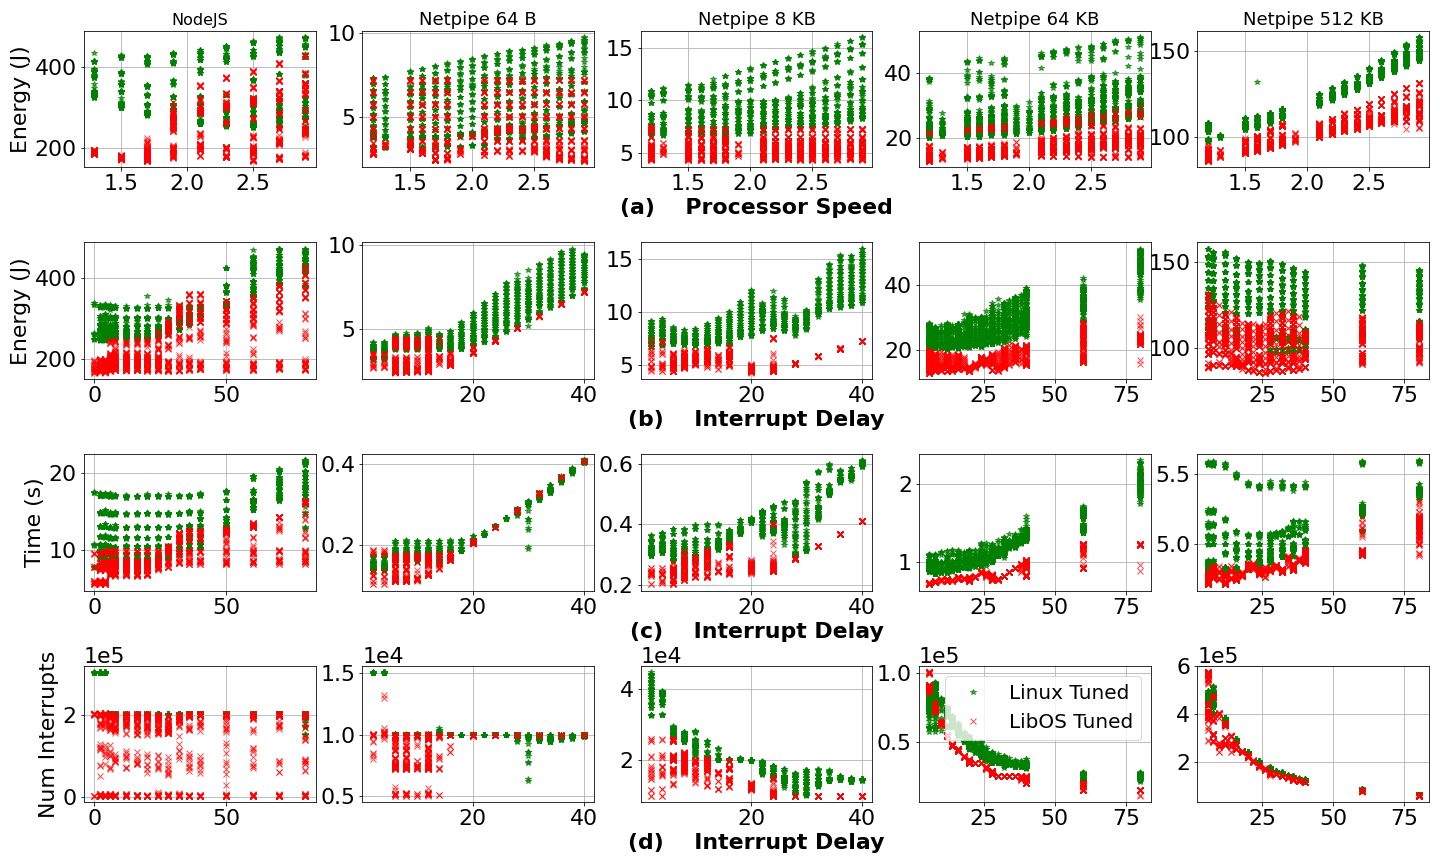
\includegraphics[width=1\textwidth]{figures/closed_detail_1.png}
\caption[]
%{\small 
{Closed loops.}
\label{fig:closed_loop_detail_1}
\end{figure*}
%This approach makes the workloads more predictable and can help smooth out diurnal variations as well~\cite{10.1145/2168836.2168842, 10.1145/2000064.2019527, oldi-study}.
As pointed out in previous studies of energy proportionality in datacenters, the nature of web-centric applications causes diurnal troughs~\cite{Barroso:2009:DCI:1643608, oldi-study, oldi-pegasus, warehouse-power, energyproportion, WebSearch} and one method with which to increase energy efficiency during these troughs is to maximize the amount of work done, typically under a given energy budget. Figure~\ref{fig:closed_loop_overview} illustrates the set of closed-loop workloads studied in our work, all of the workloads are run in a single core with a single connection, further, they enable us to explore these simple closed-loop examples in detail in settings of computationally intensive (nodejs) and across varying network bandwidth requirements (netpipe). Netpipe~\cite{snell1996netpipe} involves sending messages of identical size between two systems for a fixed number of iterations. We fix the iteration count at 5000 and show results for a range of message sizes. \footnote{We found that the 10 GB link is close to saturation when a message of size greater 700 KB is exchanged.}. NodeJS~\cite{nodejs} runs a JavaScript HTTP Webserver and consists of a single client, running the \textit{wrk}~\cite{wrk} benchmark\footnote{We modified \textit{wrk} to place a fixed request load of 100K.}, that sends web requests to a server thread for a fixed period of time. The server responds to each request with a small static payload of size 148 bytes. The library OS was ported to support baremetal NodeJS by providing OS interfaces that link with the V8~\cite{v8} JavaScript engine and libuv~\cite{libuv}. We believe these set of workloads will help to simplify the complexity which to compare and contrast the effects of slowing down in the four types of systems listed above.

\subsection{Observation-1: Speed up interrupt delay to induce polling}

\subsection{Finding-1: Slow-to-stay-busy}

\subsection{Trade-offs in when polling}
